\section{Вычислительный эксперимент} \label{sec:experiments}

    В этом разделе представлены результаты экспериментов по применению аппроксимации \texttt{JAGUAR} в различных задачах оптимизации "черного ящика". Результаты включают оптимизацию с помощью алгоритмов Франка-Вульфа как для детерминированного, так и стохастического случаев. Технические подробности и дополнительные эксперименты представлены в Приложении \ref{appendix:experiments}.

\subsection{Постановка эксперимента}

    Я рассмотрел задачу классификации моделью логистической регрессии с регуляризацией $L_2$ на множестве $Q$ вида:
    \begin{equation} \label{eq:logreg}
        \min_{w \in Q} f(w) = \frac{1}{m} \sum_{k = 1}^{m} \log \left( 1 + \exp \left( -\mathbf{y}_k \cdot (\mathbf{X} \mathbf{w})_k \right) \right) + \lambda \| \mathbf{w} \|_2^2,
    \end{equation}
    где коэффициент регуляризации $\lambda=0.05$. А также квадратичную задачу:
    \begin{equation} \label{eq:quadratic}
        \min_{w \in Q} f(w) = \| \mathbf{y} - \mathbf{X} \mathbf{w} \|^2.
    \end{equation}
    В качестве минимизирующего множества $Q$ рассматриваются симплекс $\Delta_d$ и $L_2$-шар.
    
    Для логистической регрессии \eqref{eq:logreg} использовались данные датасета mushrooms из библиотеки LibSVM \citep{chang2011libsvm}, а для квадратичной задачи \eqref{eq:quadratic} -- синтетические данные. Было показано, что использование \texttt{JAGUAR} работает лучше, чем использование базовых оценок градиентов: $l_2$-сглаживания \eqref{eq:l2_approx} и полной аппроксимации \eqref{eq:turtle_approx}.

\subsection{Детерминированный Франк-Вульф}

    В этом разделе предполагаем, что есть шум в виде округления. На рисунке \ref{fig:FW_determ} показана сходимость детерминированного алгоритма ФВ с аппроксимацией \texttt{JAGUAR} (алгоритм \ref{alg:FW}). Алгоритм значительно превосходит базовые аппроксимации, эти наблюдения подтверждают наши теоретические выводы. В этом разделе можно увидеть результаты только для $Q = \Delta_d$, эксперименты на $L_2$-шаре можно найти в приложении \ref{приложение:эксперименты}.

    \begin{figure}[H]
        \begin{center}
            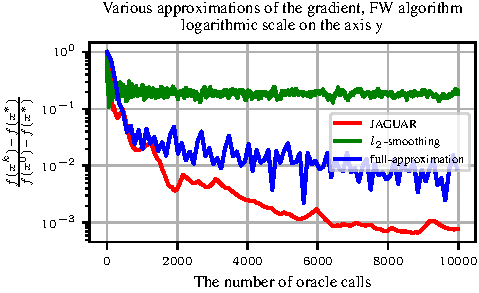
\includegraphics[width=0.49\columnwidth]{pictures/Non_stochastics_FW_LogReg_Simplex.pdf}
            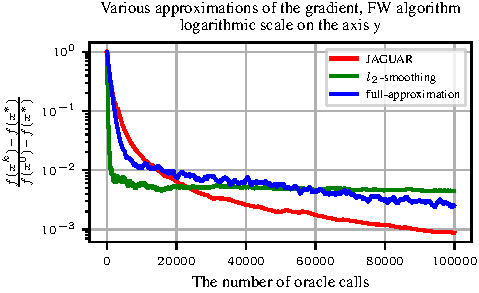
\includegraphics[width=0.49\columnwidth]{pictures/Non_stochastics_FW_Reg_Simplex.pdf}
            \caption{Сходимость алгоритма ФВ в логарифмической задаче (слева) и квадратичной задаче (справа) на множестве $Q = \Delta_d$.}
            \label{fig:FW_determ}
        \end{center}
    \end{figure}
    
    
\subsection{Стохастический Франк-Вульф}

    В этом разделе рассматривается только квадратичная задача минимизации \eqref{eq:quadratic}, однако предполагается, что есть стохастический шум в виде $\delta(x, \xi) = \xi \sim \mathcal{N}(0, \sigma^2)$, где $\sigma^2 = 0.1$. На рисунке \ref{fig:FW_determ} показана сходимость стохастического алгоритма ФВ с аппроксимацией \texttt{JAGUAR} (алгоритм \ref{alg:FW_stoch}). Случай ДОС превосходит базовые алгоритмы с большим отрывом, и эти наблюдения подтверждают наши теоретические выводы.
    В этом разделе можно увидеть результаты для $Q = \Delta_d$ и $L_2$-шара.

    \begin{figure}[H]
        \centering
            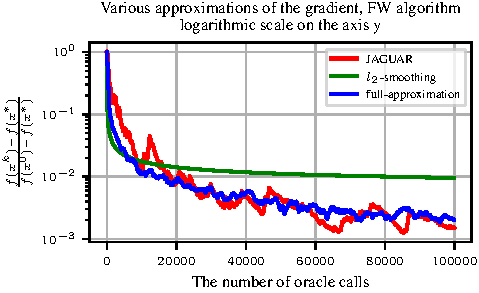
\includegraphics[width=0.49\columnwidth]{pictures/Stochastics_TPF_FW_Reg_Simplex.pdf}
            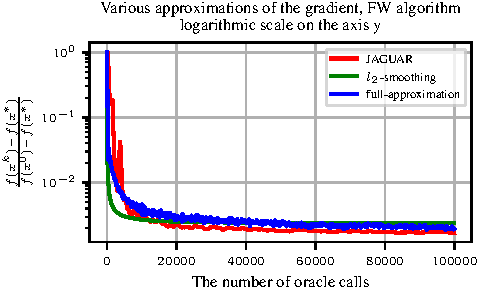
\includegraphics[width=0.49\columnwidth]{pictures/Stochastics_TPF_FW_Reg_L2.pdf}
            \caption{Сходимость алгоритма ФВ на квадратичной задаче \eqref{eq:quadratic} со стохастическим шумом на множествах $Q = \Delta_d$ (слева) и $L_2$-шаре (справа).}
        \label{fig:FW_stoch}
    \end{figure}

\textbf{Картинки будут переделаны с подписями на русском и в другом стиле}